\section{\printdate{2015/08/25} - Building GEOtop on Windows 7}\label{sec:20150825}

It's possible to build GEOtop with static and shared linking method. However, it's not possible to build the source code through Microsoft Visual Studio at the moment. So it's necessary to install Cygwin as following described.

\subsection{Install Cygwin}

Download the executable from the official web site \url{https://cygwin.com/install.html}

\begin{figure*}[h!]
  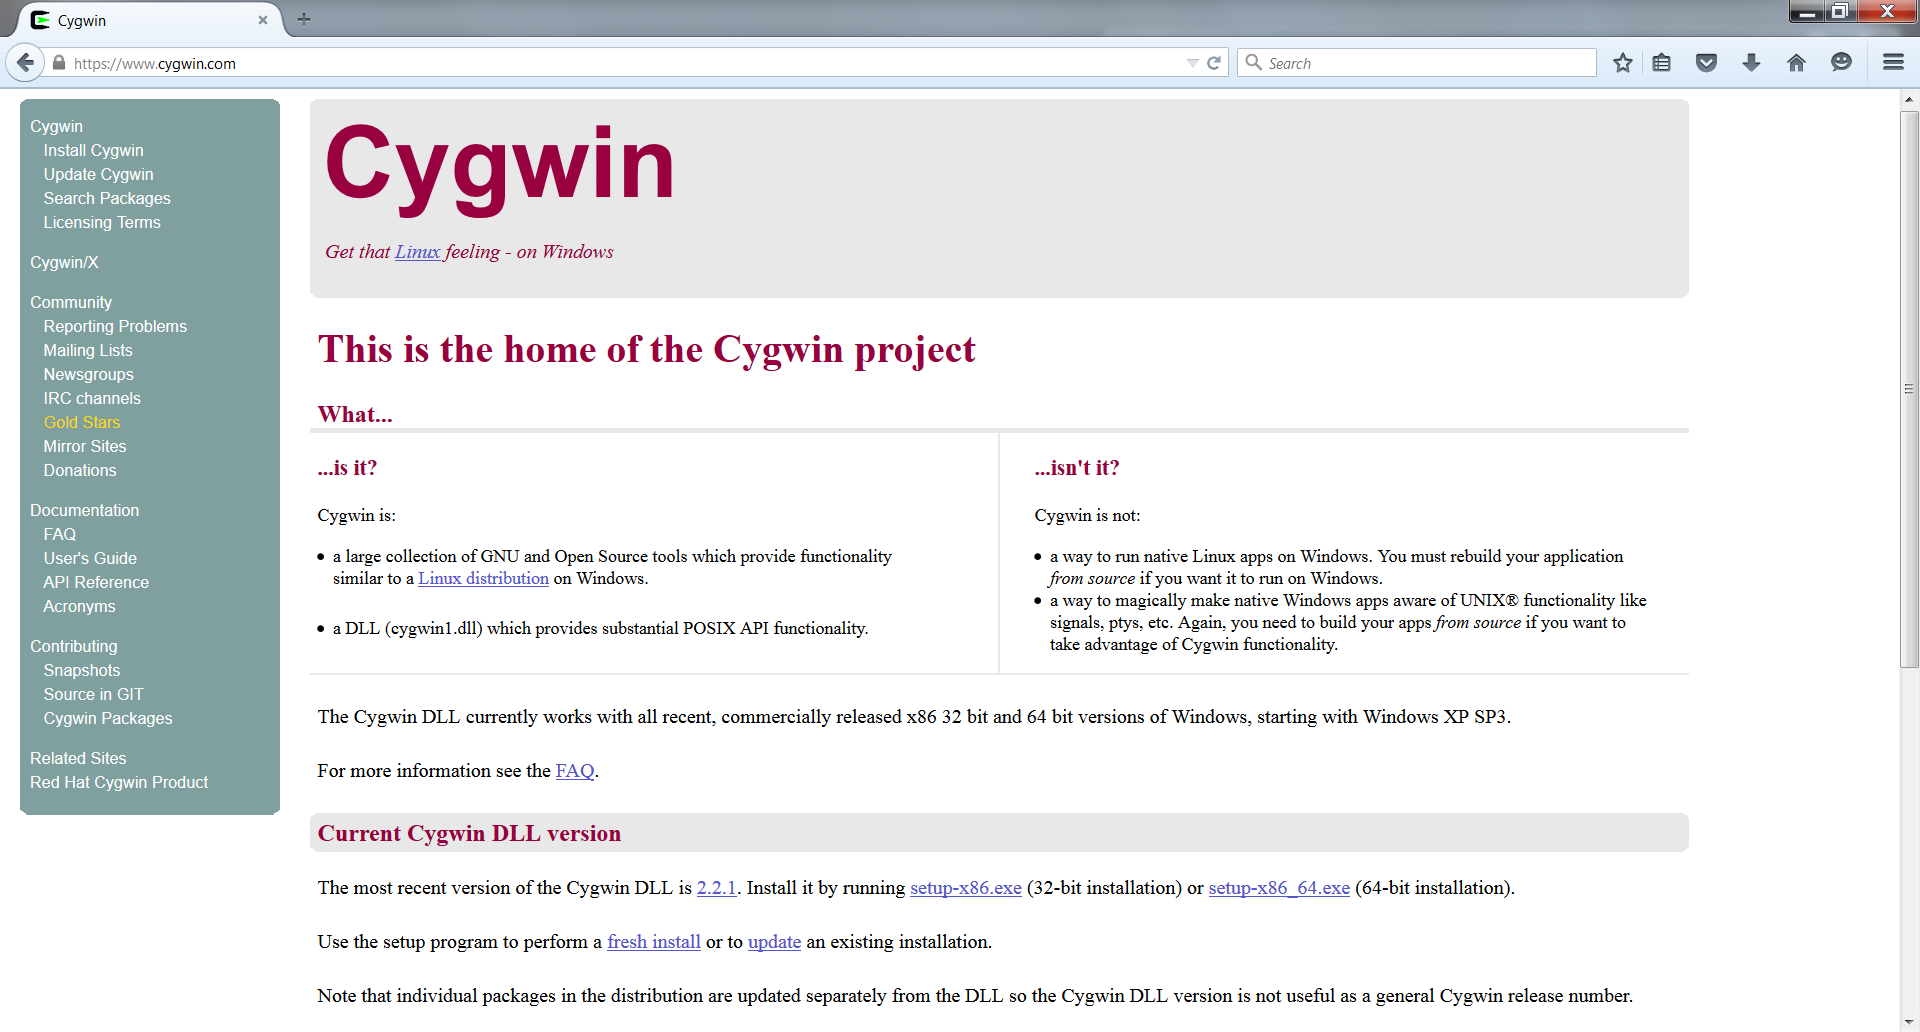
\includegraphics[width=\linewidth]{2015/Aug/25/1pic.png}
\end{figure*}

Then follow the screenshots until arriving at \textbf{Choose Download Site}

\pagebreak

\begin{figure*}[ht!]
  \centering
  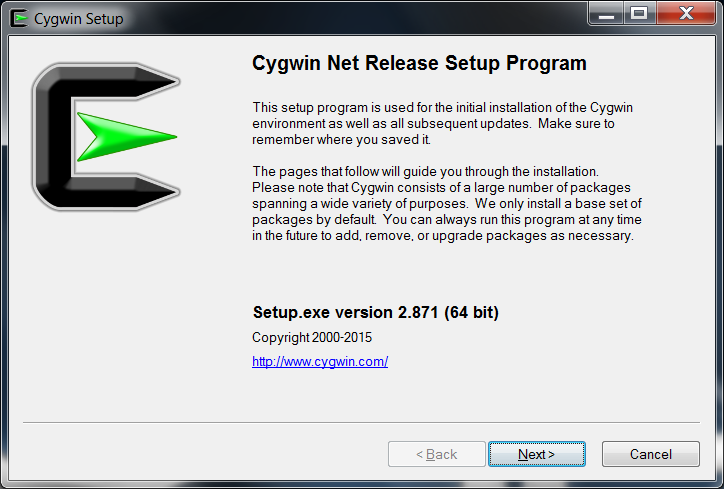
\includegraphics[width=0.7\linewidth]{2015/Aug/25/2pic.png}
\end{figure*}
\begin{figure*}[h!]
  \centering
  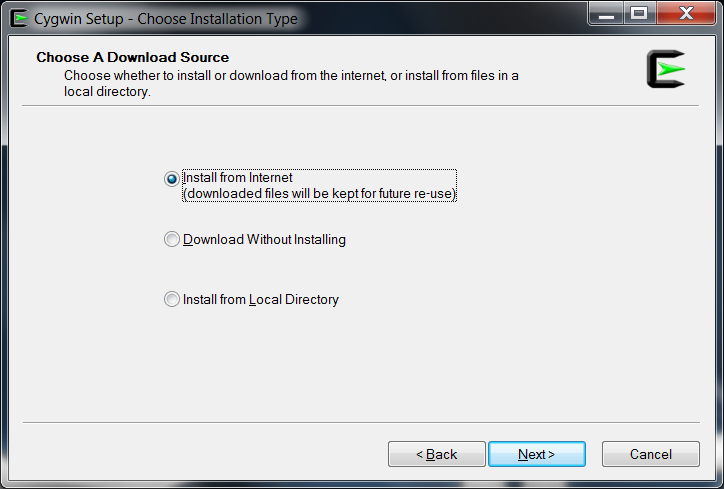
\includegraphics[width=0.7\linewidth]{2015/Aug/25/3pic.png}
\end{figure*}

\pagebreak

\begin{figure*}[ht!]
  \centering
  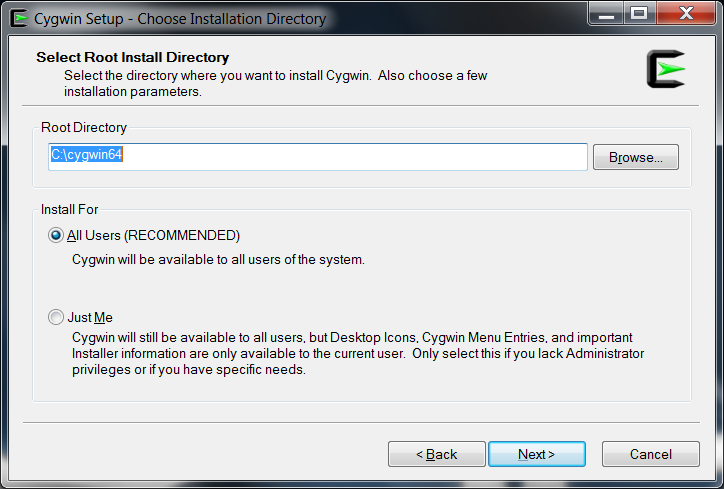
\includegraphics[width=0.7\linewidth]{2015/Aug/25/4pic.png}
\end{figure*}
\begin{figure*}[h!]
  \centering
  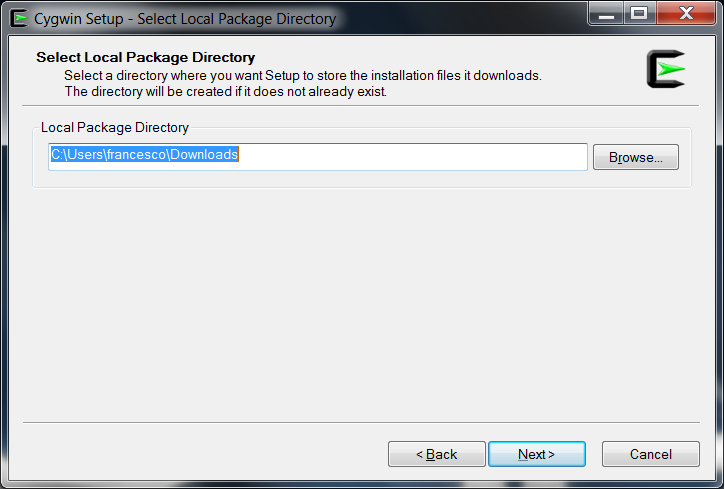
\includegraphics[width=0.7\linewidth]{2015/Aug/25/5pic.png}
\end{figure*}

\pagebreak

\begin{figure*}[ht!]
  \centering
  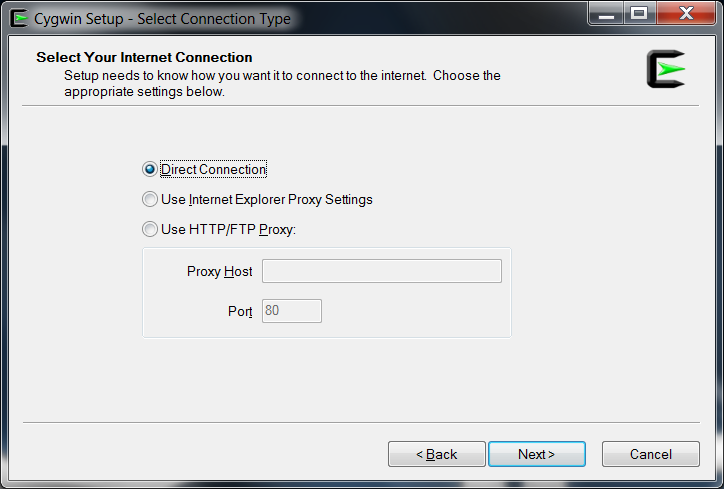
\includegraphics[width=0.7\linewidth]{2015/Aug/25/6pic.png}
\end{figure*}
\begin{figure*}[h!]
  \centering
  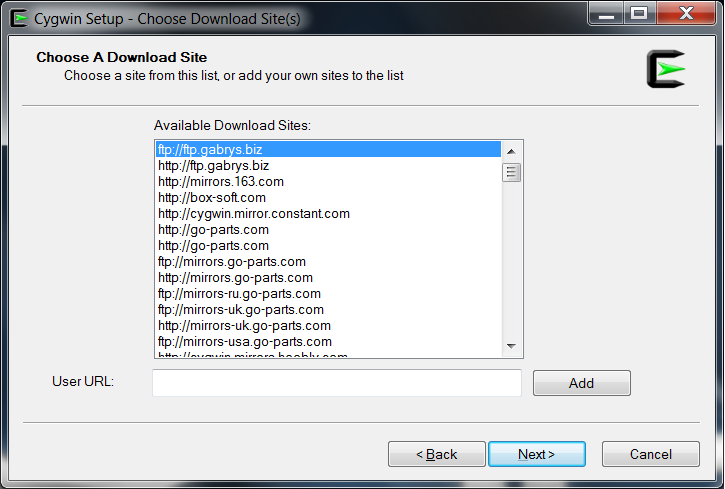
\includegraphics[width=0.7\linewidth]{2015/Aug/25/7pic.png}
\end{figure*}

\pagebreak

Now, choose a repository from which download the packages to install. Then click \textcolor{blue}{Next} and you should see a window like the following

\begin{figure*}[h]
  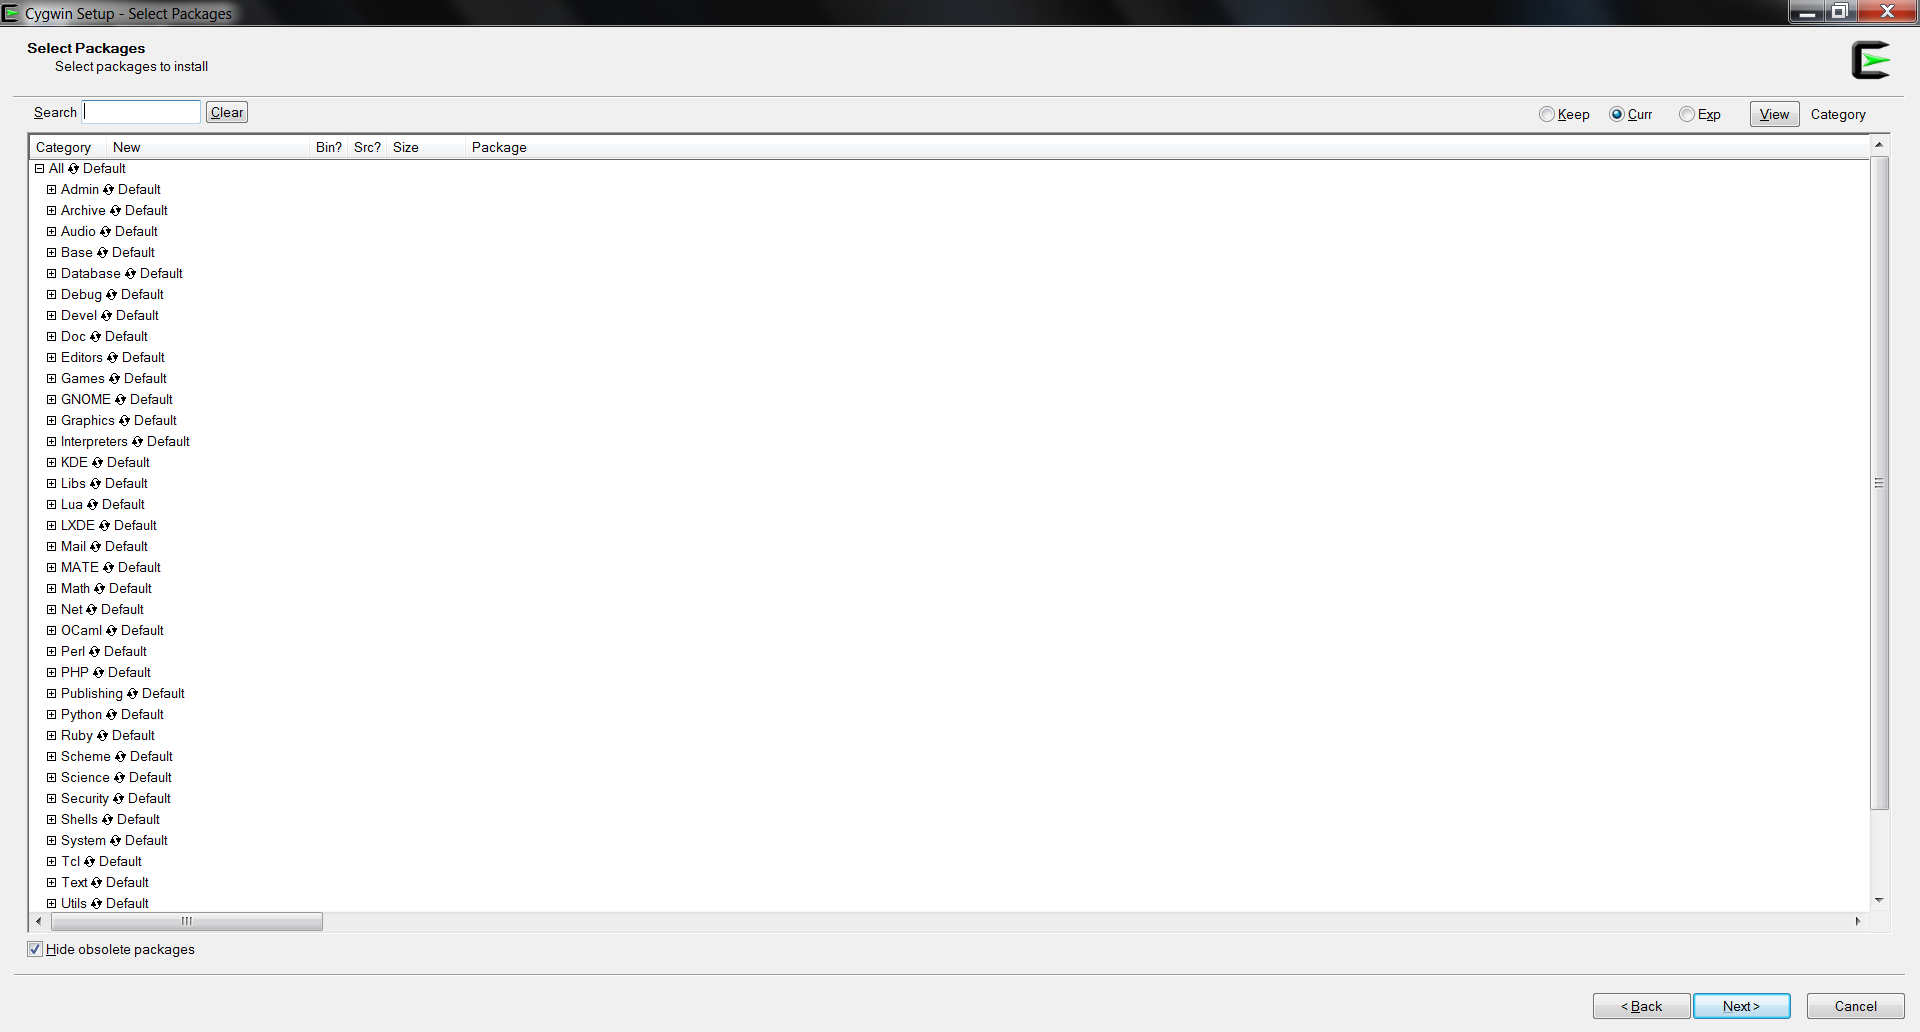
\includegraphics[width=\linewidth]{2015/Aug/25/8pic.png}
\end{figure*}

\noindent Expand the \textbf{Archive} section and select the following packages

\begin{itemize}
\item \textbf{libbz2-devel}
\end{itemize}

\noindent Expand the \textbf{Development} section and select the following packages

\begin{itemize}
\item \textbf{autoconf2.5}
\item \textbf{cmake}
\item \textbf{cmake-gui}
\item \textbf{gcc-core}
\item \textbf{gcc-g++}
\item \textbf{git}
\item \textbf{make}
\item \textbf{patch}
\end{itemize}

% \noindent Expand the \textbf{Libs} section and select the following packages

% \begin{itemize}
% \item \textbf{zlib}
% \item \textbf{zlib-devel}
% \item \textbf{zlib0}
% \end{itemize}

\pagebreak

Now type \inline{proj} in the \textbf{Search area}

\begin{figure}[h]
  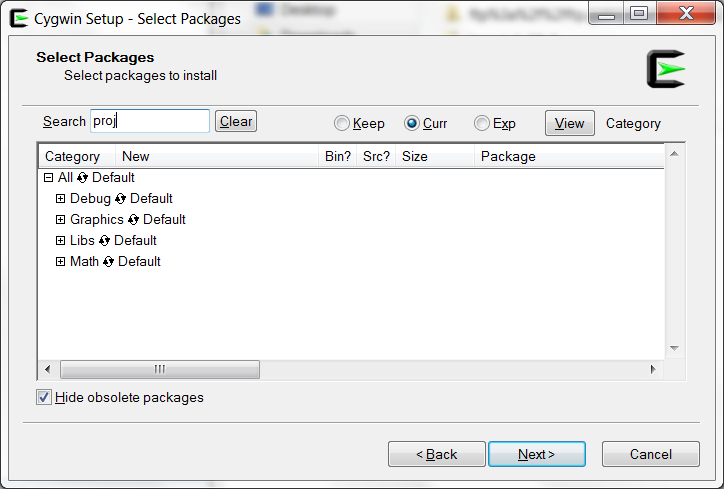
\includegraphics[width=\textwidth]{2015/Aug/25/proj1.png}
\end{figure}

Expand the section \inline{Libs}

\begin{figure}[h]
  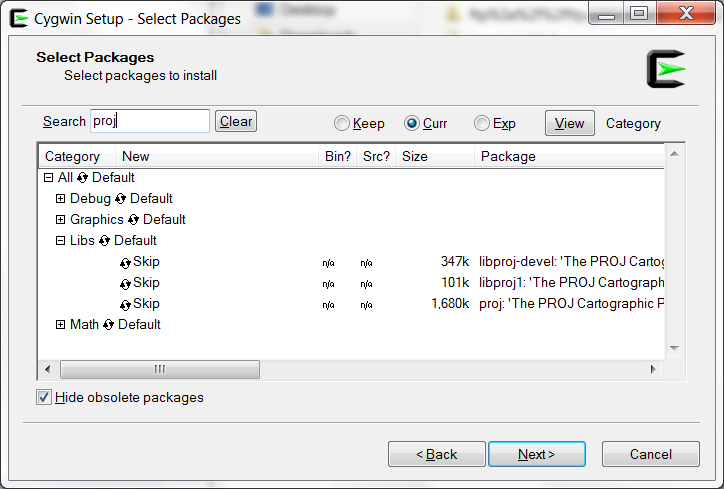
\includegraphics[width=\linewidth]{2015/Aug/25/proj2.png}
\end{figure}

Click on \inline{Skip} on the three proj libraries:

\begin{itemize}
\item libproj-devel
\item libproj1
\item proj
\end{itemize}

\pagebreak

\begin{figure}[h]
  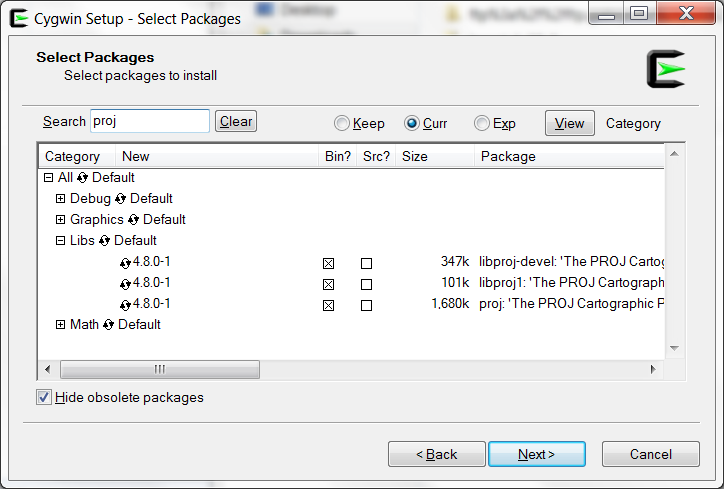
\includegraphics[width=\linewidth]{2015/Aug/25/proj3.png}
\end{figure}

Then click on \inline{Next}

\begin{figure}[h]
  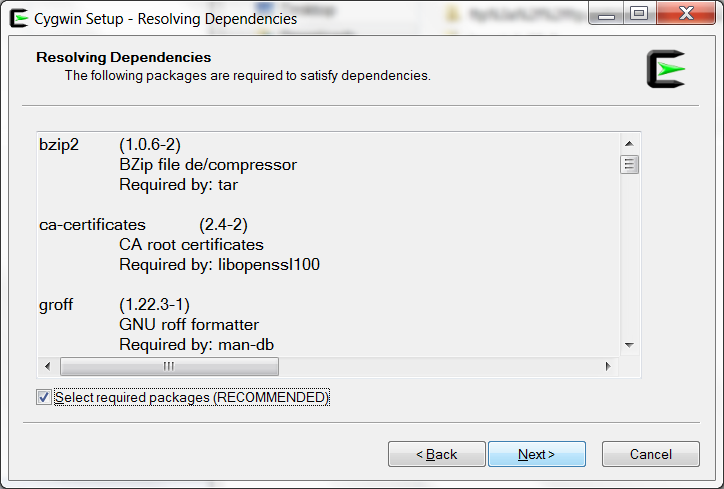
\includegraphics[width=\linewidth]{2015/Aug/25/proj4.png}
\end{figure}

Then click on \inline{Next} again, in order to install all the required dependencies. At the end of the installation, you should find an icon on the Desktop and one on the Start Menu.

\subsection{Building GEOtop: static linking}

First of all, open the Cygwin terminal (a link should be done on the Desktop). Enter inside your user home typing:

\begin{lstlisting}[style=bashStyle]
$ cd /cygdrive/c/Users/<user>
\end{lstlisting} %$

where \inline{<user>} is your username. Now create a folder where put the source codes, e.g. \inline{src}, and enter into. % Then, cloning the \textbf{PROJ.4} source code from \url{https://github.com/francescoS/proj4.7.0_patched} github repository through \inline{git} command line. Enter into the main PROJ.4 directory.

% \begin{lstlisting}[style=bashStyle]
% $ mkdir src
% $ cd src/

% # clone the PROJ.4
% $ git clone https://github.com/francescoS/proj4.7.0_patched
% $ cd proj.4.7.0_patched/
% \end{lstlisting}

% The use of a non official github repository is due to the lack of compatibility of PROJ.4 with Cygwin. This doesn't mean that you can't build the library, but this doesn't properly work with MeteoIO and then with GEOtop. So, we are using an old version (4.7.0) patched in order to properly work under Cygwin. To statically build the library, follow these simple steps.

% \begin{lstlisting}[style=bashStyle]
% $ ./configure --enable-shared=off
% $ make
% $ make install
% \end{lstlisting} %$
% It's necessary to explicitly say to the compiler that we want only static library more for future comfort: building MeteoIO and GEOtop, CMake firt of all looks for dependencies built as shared libraries. So that, we should change the settings in the cmake-gui to link to the static version of the library. But, if no shared libraries have been built, cmake is going to link the only libraries present, in our case the static ones.

Now you need the MeteoIO source code and then you have to build it. Unfortunately, in order to make it works with Cygwin you should apply a patch to the official version. I created the patched version of the MeteoIO 2.4.2 source code and then I uploaded it on GitHub, so you can easily clone and build it.

\begin{lstlisting}[style=bashStyle]
# download MeteoIO from the unofficial repo
$ git clone https://github.com/francescoS/MeteoIO-2.4.2_patched
$ cd MeteoIO-2.4.2_patched
\end{lstlisting}

\begin{lstlisting}[style=bashStyle]
$ ccmake .
# type 'c' to configure, and if you get a warning message just type 'e' to exit
\end{lstlisting} %$

\begin{figure}[h]
  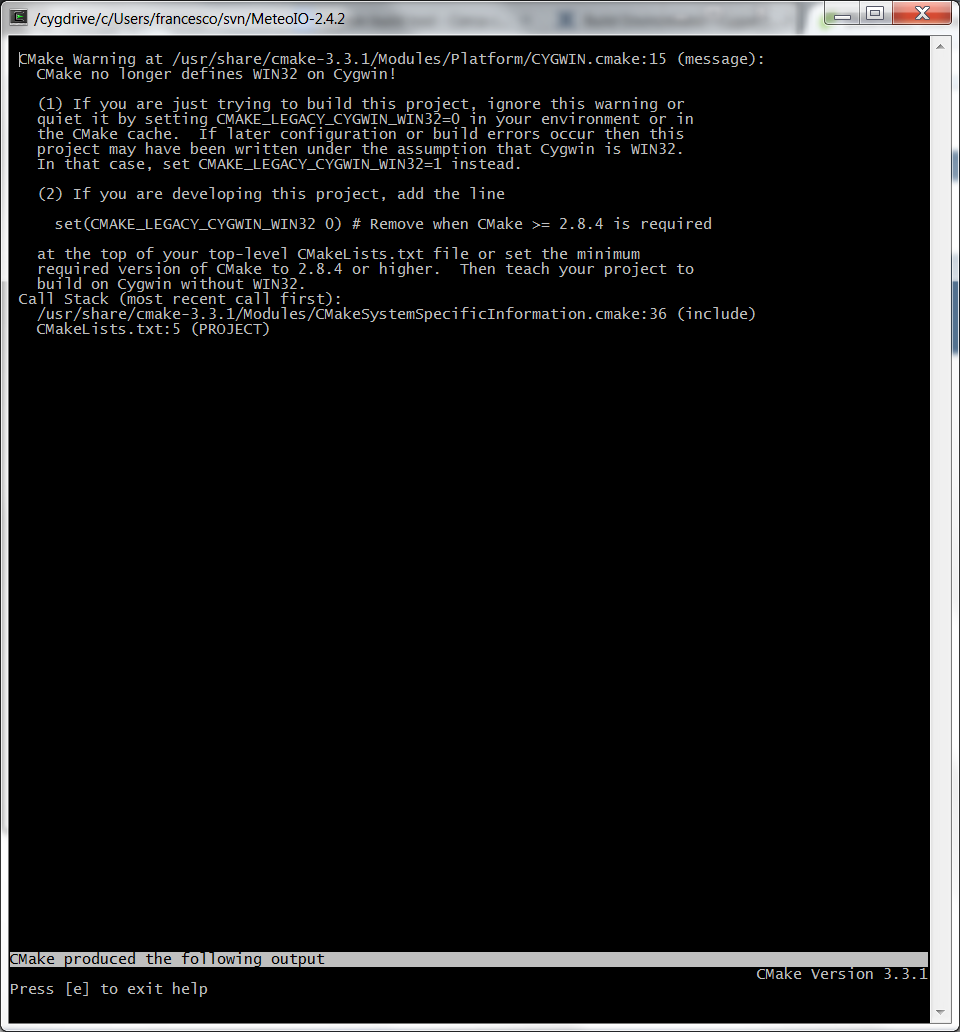
\includegraphics[width=\linewidth]{2015/Aug/25/9pic.png}
\end{figure}

\pagebreak

\begin{lstlisting}[style=bashStyle]
# set build_shared_libs OFF build_static_libs ON
\end{lstlisting}

\begin{figure}[h]
  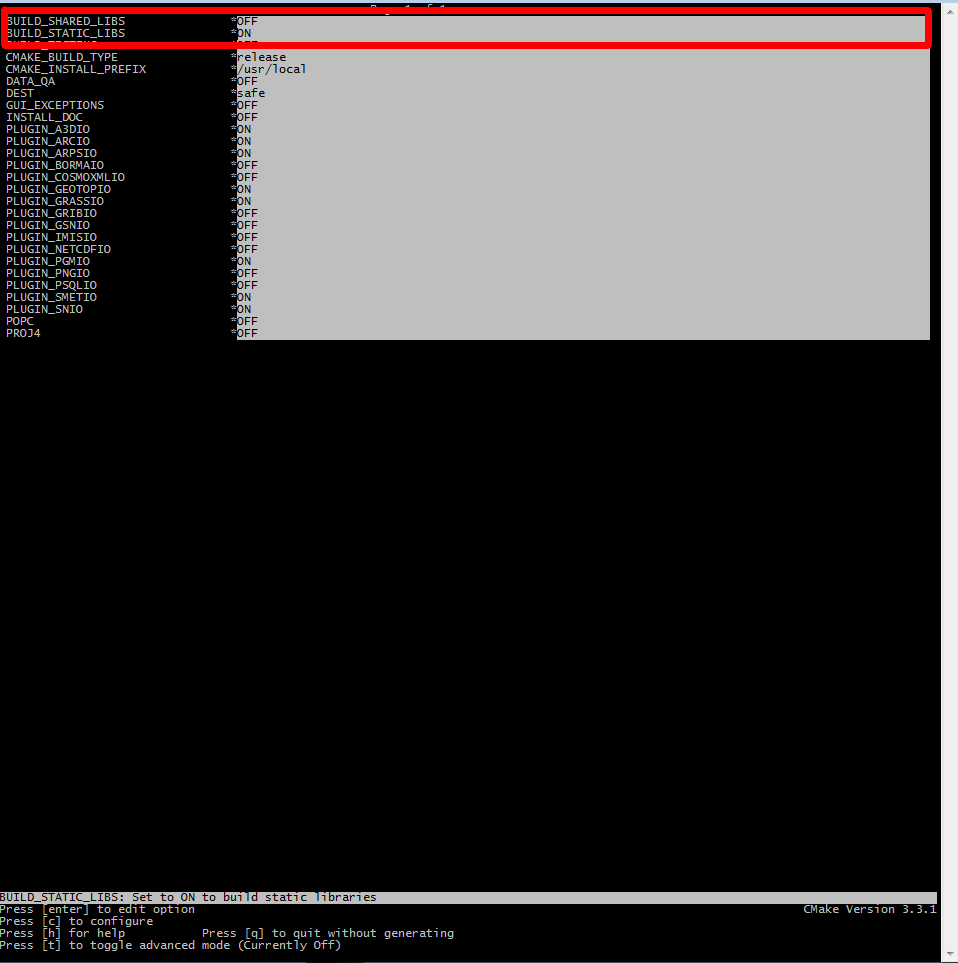
\includegraphics[width=\linewidth]{2015/Aug/25/10pic.png}
\end{figure}

\pagebreak

\begin{lstlisting}[style=bashStyle]
# set the proj tag ON
\end{lstlisting}

\begin{figure}[h]
  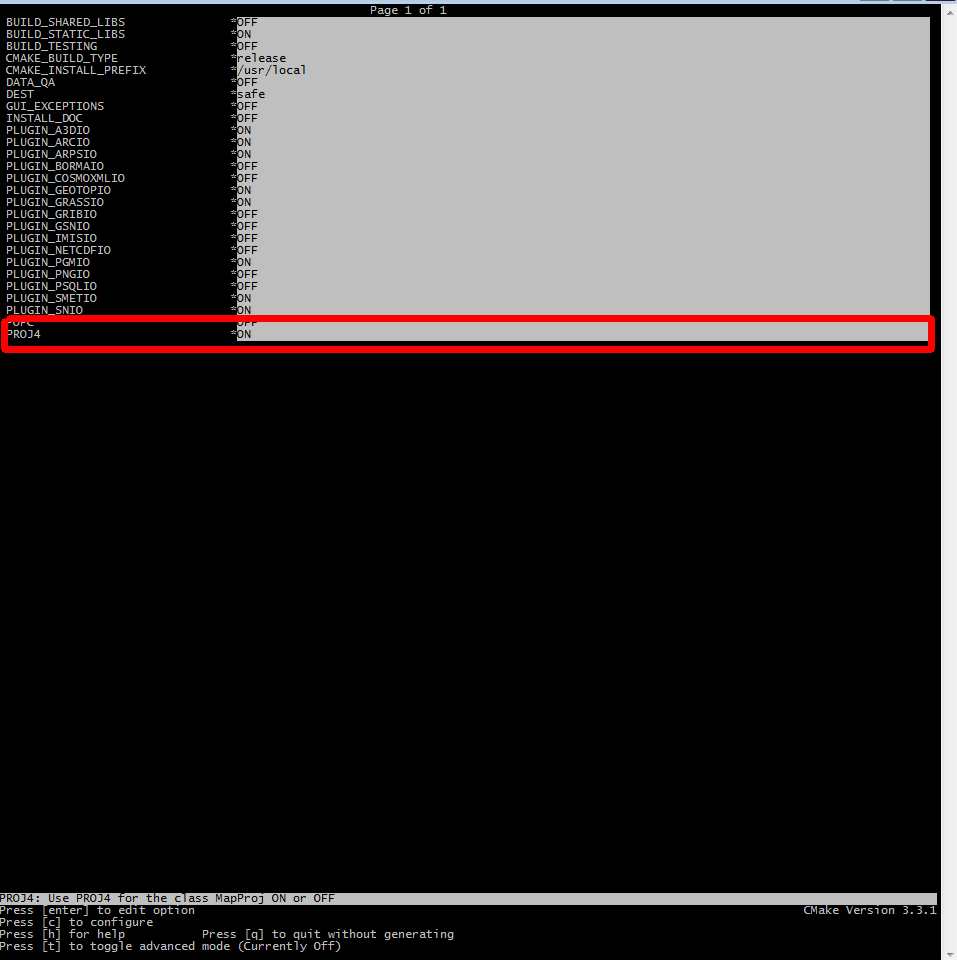
\includegraphics[width=\linewidth]{2015/Aug/25/11pic.png}
\end{figure}

\begin{lstlisting}[style=bashStyle]
# type 'c' to configure, 'c' to configure, 'g' to generate
$ make
$ make install
\end{lstlisting} %$

Now you have to build the \textbf{Boost} library. First of all, you can get it from \url{http://sourceforge.net/projects/boost/files/boost/1.58.0/}, then move the package inside the \inline{src} folder. Extract the source code and then enter into the folder

\begin{lstlisting}[style=bashStyle]
$ tar -xzvf boost_1_58_0.tar.gz
$ cd boost_1_58_0/
\end{lstlisting}

Now, to configure and then build and install the \textbf{Boost} library, type

\begin{lstlisting}[style=bashStyle]
$ ./bootstrap.sh --with-libraries=filesystem,system,iostreams,regex,program_options,test
$ ./bjam link=static install
\end{lstlisting} %$

Now, the last step is building GEOtop. You can clone it from the GitHub repository, inside the \inline{src} directory

\begin{lstlisting}[style=bashStyle]
$ cd ~/src
$ git clone https://github.com/francescoS/geotop
\end{lstlisting}

It's not possible to build the \textbf{master}-brach with static linking. Therefore, you have to switch branch

\begin{lstlisting}[style=bashStyle]
$ git checkout cmake_redesign
\end{lstlisting} %$

Now, start the building

\begin{lstlisting}[style=bashStyle]
$ ccmake .
# press 'c' to configure
# press 'e' to exit (even if warining is shown)
# switch static to ON
# press 'c' to configure
# press 'e' after static linking mode shown
# press 'c' to configure
# press 'e' after static linking mode shown
# press 'g' to generate
\end{lstlisting} %$

\begin{lstlisting}[style=bashStyle]
$ make
\end{lstlisting} %$

\begin{lstlisting}[style=bashStyle]
$ make install
\end{lstlisting} %$

adding \inline{C:\cygwin(64 if your have 64bit pc)\bin} to environmental variables or you can simply move the executable wherever you want

\subsection{Building GEOtop: shared linking}

Unfortunately, I'm not able to build \textbf{Boost} (1.58.0 - 1.59.0) under Windows 7 with shared linking. I get error building iostrems module.
